\chapter{La mer de Dirac, la masse des fermions et les spineurs à quatre composantes}

\section{Fermions se déplaçant vers la droite et mer de Dirac}

L’équation de Dirac est une équation pour les fermions. Les bosons relativistes satisfont d’autres équations, comme l’équation de Klein--Gordon ou les équations de Maxwell. L’exemple le plus simple se situe dans une dimension spatiale et décrit d’abord des particules et des antiparticules qui ne peuvent se déplacer que vers la droite.

Commençons par une onde plane,
\begin{equation}
\psi(x,t)=\psi_0 e^{i(kx-\omega t)}.
\end{equation}
Sa vitesse de phase est
\begin{equation}
v_{\mathrm{ph}}=\frac{\omega}{k}.
\end{equation}
Les signes de \(k\) et de \(\omega\) sont importants. S’ils sont identiques, la phase se déplace vers la droite ; s’ils sont opposés, elle se déplace vers la gauche. Lorsque \(\omega\) est proportionnel à \(k\), les vitesses de phase et de groupe coïncident :
\begin{equation}
v_{\mathrm{g}}=\frac{d\omega}{dk}=\frac{\omega}{k}.
\end{equation}

Considérons l’équation du premier ordre
\begin{equation}
\frac{\partial\psi}{\partial x}
+
\frac{\partial\psi}{\partial t}
=0.
\end{equation}
En y substituant l’onde plane, on obtient
\begin{equation}
ik\psi-i\omega\psi=0,
\end{equation}
d’où
\begin{equation}
\omega=k.
\end{equation}
L’onde se déplace donc vers la droite. Il est utile de noter le champ en conséquence :
\begin{equation}
\frac{\partial\psi_R}{\partial t}
=
-\frac{\partial\psi_R}{\partial x}.
\end{equation}

En rétablissant la vitesse de la lumière, on obtient la forme dimensionnelle
\begin{equation}
\frac{\partial\psi_R}{\partial x}
+
\frac{1}{c}\frac{\partial\psi_R}{\partial t}
=0,
\end{equation}
donc
\begin{equation}
\omega=ck.
\end{equation}
Désormais, \(c=1\). Avec \(\hbar=1\), \(\omega\) est aussi l’énergie d’un quantum.

\begin{figure}[htbp]
\centering
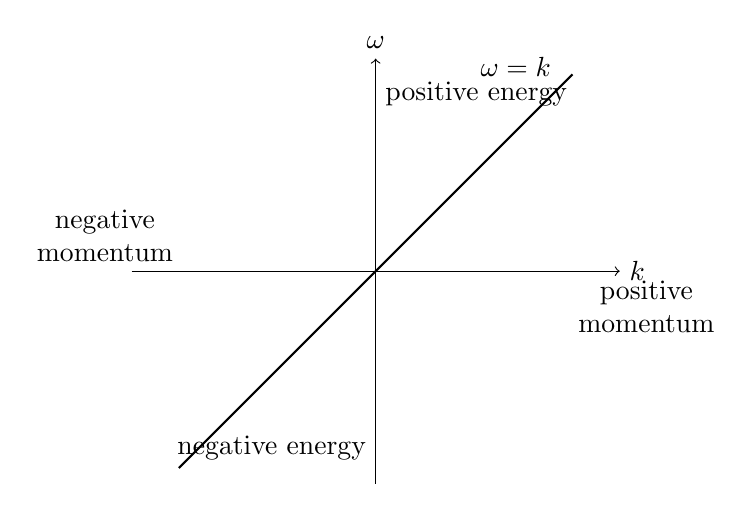
\begin{tikzpicture}[scale=1.0]
\draw[->] (-3.1,0) -- (3.1,0) node[right] {$k$};
\draw[->] (0,-2.7) -- (0,2.7) node[above] {$\omega$};
\draw[thick] (-2.5,-2.5) -- (2.5,2.5);
\node[above left] at (2.35,2.35) {$\omega=k$};
\node[below right,align=center] at (2.45,0) {positive\\momentum};
\node[above left,align=center] at (-2.45,0) {negative\\momentum};
\node[right] at (0,2.25) {positive energy};
\node[left] at (0,-2.25) {negative energy};
\end{tikzpicture}
\caption{La relation de dispersion sans masse pour les modes se déplaçant vers la droite, \(\omega=k\), comporte des branches d’énergie positive et négative.}
\end{figure}

Cette droite a une conséquence grave. Une valeur positive de \(k\) donne une énergie positive, tandis qu’une valeur négative de \(k\) donne une énergie négative. Les deux parties décrivent néanmoins des ondes se déplaçant vers la droite, car \(\omega/k=1\) sur toute la droite.

Un électron placé sur la branche d’énergie positive pourrait tomber vers un état inférieur, émettre un photon d’énergie positive, retomber, puis continuer à descendre dans le spectre : un degré plus bas, puis un autre, puis encore un autre. Aucun électron ne serait stable. Plus grave encore, le monde abaisserait son énergie en produisant toujours davantage d’électrons d’énergie négative.

Le principe d’exclusion des fermions apporte la solution. Remplissons tous les états électroniques d’énergie négative. Aucun second électron ne peut occuper un état déjà occupé ; le secteur d’énergie négative entièrement rempli empêche donc une chute illimitée. Ce secteur rempli constitue la mer de Dirac, et son état entièrement rempli est l’état fondamental, ou le vide.

\begin{classroomqa}
\lecturetimestamp{00:07:19}
\audiencequestion{Existe-t-il une infinité d’états d’énergie négative plus basse ?}
\lecturerresponse{Oui. Avec des moments discrets, le spectre ressemble à un escalier sans fin ; avec des moments continus, à une pente continue. Le remplissage de la mer d’énergie négative empêche un électron de descendre indéfiniment, même si une transition vers un état inférieur, avec émission d’un photon, peut encore avoir lieu lorsqu’un tel état est inoccupé.}
\end{classroomqa}

Cela explique pourquoi une équation présentant ce spectre doit être quantifiée comme une théorie fermionique. Si les quanta étaient des bosons, un nombre arbitrairement grand d’entre eux pourrait occuper le même état inférieur, et le remplissage du secteur d’énergie négative ne stabiliserait pas le vide.

L’image de la mer remplie fait aussi apparaître les antiparticules. Dans le vide, tous les niveaux d’énergie négative sont occupés et tous ceux d’énergie positive sont vides. Un électron peut être promu de n’importe quel niveau d’énergie négative occupé vers n’importe quel niveau d’énergie positive inoccupé ; les niveaux initial et final n’ont pas besoin d’être symétriques.

\begin{figure}[htbp]
\centering
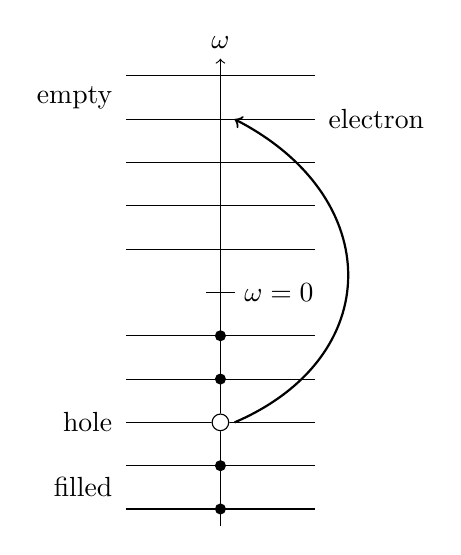
\begin{tikzpicture}[x=1cm,y=0.55cm]
\draw[->] (0,-5.4) -- (0,5.4) node[above] {$\omega$};
\draw (-0.18,0) -- (0.18,0) node[right] {$\omega=0$};
\foreach \y in {-5,-4,-3,-2,-1} {
  \draw (-1.2,\y) -- (1.2,\y);
  \fill (0,\y) circle (2pt);
}
\foreach \y in {1,2,3,4,5} {
  \draw (-1.2,\y) -- (1.2,\y);
}
\draw[->,thick] (0.18,-3) .. controls (2.1,-1.5) and (2.1,2.2) .. (0.18,4);
\draw[white,fill=white] (0,-3) circle (3pt);
\draw (0,-3) circle (3pt);
\node[left] at (-1.25,-3) {hole};
\node[left] at (-1.25,-4.5) {filled};
\node[left] at (-1.25,4.5) {empty};
\node[right] at (1.25,4) {electron};
\end{tikzpicture}
\caption{La promotion d’un électron d’énergie négative qui occupait un état produit un électron d’énergie positive et laisse un trou dans la mer remplie.}
\end{figure}

Retirer un électron d’énergie négative augmente l’énergie par rapport au vide ; le trou a donc une énergie positive. Sur la branche \(\omega=k\), l’électron retiré avait également un moment négatif. En retirant un moment négatif, on laisse un excès positif de moment : le trou a donc un moment positif. Si l’on prend la charge de l’électron comme négative, l’électron manquant a une charge positive. Le trou est ainsi une antiparticule d’énergie et de moment positifs, tandis que l’électron promu a une charge négative, une énergie positive et un moment positif. Dans cette théorie à une seule branche, toutes les excitations réelles se déplacent vers la droite.

Le champ \(\psi_R\) est construit à partir d’opérateurs fermioniques de création et d’annihilation. L’interprétation en termes de particule et de trou concerne donc les quanta créés et éliminés par le champ, et pas seulement une onde classique.

Il subsiste une asymétrie. La mer des modes se déplaçant vers la droite contient des états d’énergie négative et de moment négatif. Son moment total formel est immense et dirigé vers la gauche. On peut définir par soustraction le moment du vide comme étant nul, mais l’état reste déséquilibré dans sa structure : particules et antiparticules ne se déplacent que vers la droite, tandis que le vide rempli est constitué d’états de moment négatif.

\section{La branche des modes se déplaçant vers la gauche et un vide équilibré}

Pour équilibrer les modes de gauche et de droite, il faut un second champ indépendant, doté de ses propres opérateurs de création et d’annihilation. Supposons qu’il satisfasse
\begin{equation}
\frac{\partial\psi_L}{\partial t}
=
+\frac{\partial\psi_L}{\partial x}.
\end{equation}
Pour la même forme d’onde plane,
\begin{equation}
-i\omega\psi_L=ik\psi_L,
\end{equation}
d’où
\begin{equation}
\omega=-k.
\end{equation}
Cette seconde droite est l’image miroir de \(\omega=k\). Sa branche d’énergie positive décrit des particules se déplaçant vers la gauche, et sa branche d’énergie négative doit elle aussi être remplie.

\begin{figure}[htbp]
\centering
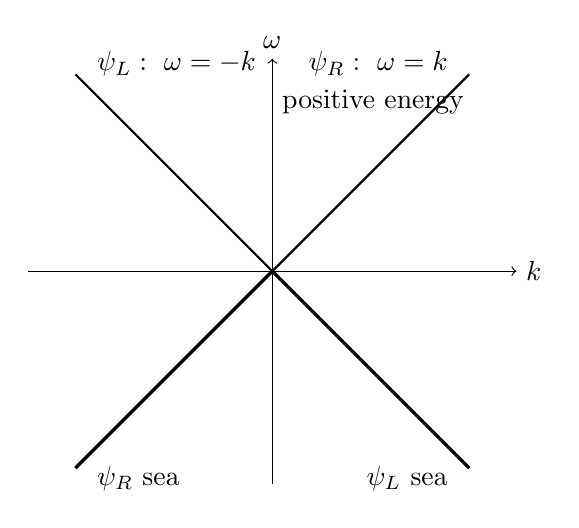
\begin{tikzpicture}[scale=1.0]
\draw[->] (-3.1,0) -- (3.1,0) node[right] {$k$};
\draw[->] (0,-2.7) -- (0,2.7) node[above] {$\omega$};
\draw[thick] (-2.5,-2.5) -- (2.5,2.5);
\draw[thick] (-2.5,2.5) -- (2.5,-2.5);
\draw[very thick] (-2.5,-2.5) -- (0,0);
\draw[very thick] (0,0) -- (2.5,-2.5);
\node[above left] at (2.35,2.35) {$\psi_R:\ \omega=k$};
\node[above right] at (-2.35,2.35) {$\psi_L:\ \omega=-k$};
\node[right] at (0,2.15) {positive energy};
\node[below right] at (-2.35,-2.35) {$\psi_R$ sea};
\node[below left] at (2.35,-2.35) {$\psi_L$ sea};
\end{tikzpicture}
\caption{Des champs indépendants pour les modes de droite et de gauche donnent des branches sans masse symétriques ; les deux demi-branches d’énergie négative sont remplies dans le vide.}
\end{figure}

Une fois les deux mers d’énergie négative remplies, les états occupés se déplaçant vers la gauche sont aussi nombreux que ceux se déplaçant vers la droite. Leurs moments dans le vide se compensent. Les excitations particulaires et les trous peuvent désormais se déplacer dans les deux directions.

\begin{classroomqa}
\lecturetimestamp{00:15:58}
\audiencequestion{Peut-on traiter le problème des énergies négatives sans postuler des états remplis et des trous ?}
\lecturerresponse{On peut reformuler la même théorie. On peut appeler un état électronique d’énergie négative rempli un état d’antiparticule vide ; le langage physique ne fait alors intervenir que des particules et des antiparticules d’énergie positive. L’image de la mer remplie reste un moyen utile de vérifier la cohérence, à la manière d’une bande remplie dans un métal : retirer un électron y produit un trou, tandis que promouvoir un électron produit à la fois une particule et un trou.}
\end{classroomqa}

Les excitations étudiées jusqu’ici sont sans masse. Leurs relations de dispersion sont linéaires et leurs vitesses ont pour module \(1\) : elles se déplacent donc à la vitesse de la lumière. La question suivante est de savoir comment leur donner une masse.

\section{Deux composantes et le terme de masse}

Combinons d’abord les deux champs en une colonne :
\begin{equation}
\Psi=
\begin{pmatrix}
\psi_R\\
\psi_L
\end{pmatrix}.
\end{equation}
Il ne s’agit au départ que d’une notation compacte pour deux équations indépendantes. Définissons
\begin{equation}
\alpha=
\begin{pmatrix}
1&0\\
0&-1
\end{pmatrix}.
\end{equation}
Les équations des modes se déplaçant vers la droite et vers la gauche prennent alors la forme
\begin{equation}
\frac{\partial\Psi}{\partial t}
=
-\alpha\frac{\partial\Psi}{\partial x}.
\end{equation}

\begin{figure}[htbp]
\centering
\includegraphics[width=0.78\textwidth]{lecture_06_figure_02.png}
\caption{Les champs \(\psi_R\) et \(\psi_L\) forment un spineur à deux composantes, et \(\alpha\) distingue les deux branches sans masse.}
\lectureframe{00:20:36}
\end{figure}

Pour une onde plane, les opérateurs
\begin{equation}
i\partial_t
\quad\hbox{and}\quad
-i\partial_x
\end{equation}
renvoient respectivement \(\omega\) et \(k\). On peut donc abréger l’équation matricielle ainsi :
\begin{equation}
\omega=\alpha k.
\end{equation}
Pour la composante supérieure, cela signifie \(\omega=k\) ; pour la composante inférieure, cela signifie \(\omega=-k\). Cette notation condense les deux équations, mais n’introduit aucune nouvelle physique.

Les électrons ne sont pas sans masse et ne se déplacent pas à la vitesse de la lumière. Une formule tentante pour leur énergie est l’énergie cinétique non relativiste \(k^2/(2m)\), mais elle ne peut pas servir de point de départ ici : la limite sans masse concerne déjà un mouvement à la vitesse de la lumière. La relation relativiste est
\begin{equation}
\omega^2=k^2+m^2,
\end{equation}
ou, en incluant les deux branches d’énergie,
\begin{equation}
\omega=\pm\sqrt{k^2+m^2}.
\end{equation}
Lorsque \(m=0\), on retrouve \(\omega=k\) et \(\omega=-k\).

\begin{classroomqa}
\lecturetimestamp{00:25:23}
\audiencequestion{Utilise-t-on des unités où \(c=1\), et comment obtient-on la vitesse d’une particule massive ?}
\lecturerresponse{La vitesse d’un paquet d’ondes est sa vitesse de groupe, \(v_{\mathrm g}=d\omega/dk=k/\sqrt{k^2+m^2}\) sur la branche d’énergie positive. La relation de dispersion donne donc elle-même la diminution de la vitesse, qui devient inférieure à \(c=1\) pour une particule massive.}
\end{classroomqa}

\begin{classroomqa}
\lecturetimestamp{00:26:29}
\audiencequestion{Dans l’écriture abrégée \(\omega=\alpha k\), \(\omega\) est-il un vecteur ou une matrice ?}
\lecturerresponse{Cette écriture abrégée désigne une équation opératorielle agissant sur la fonction d’onde à deux composantes. Ici, \(\omega\) désigne \(i\partial_t\), \(k\) désigne \(-i\partial_x\) et \(\alpha\) est la matrice qui agit sur l’indice de composante. Les symboles scalaires \(\omega\) et \(k\) ne deviennent leurs valeurs propres numériques que pour une onde plane.}
\end{classroomqa}

Conservons une équation du premier ordre et essayons la plus simple des extensions dépendant de la masse :
\begin{equation}
\omega=\alpha k+\beta m.
\end{equation}
L’objet \(\beta\) doit être une matrice, puisqu’il agit sur le même champ à deux composantes que \(\alpha\). Sa structure algébrique se déduit en élevant au carré :
\begin{align}
\omega^2
&=(\alpha k+\beta m)(\alpha k+\beta m)\\
&=\alpha^2k^2+\beta^2m^2
+\alpha\beta\,km+\beta\alpha\,mk\\
&=\alpha^2k^2+\beta^2m^2
+(\alpha\beta+\beta\alpha)km.
\end{align}
Pour obtenir \(k^2+m^2\) pour toutes les valeurs de \(k\) et de \(m\), il faut imposer
\begin{equation}
\alpha^2=I,
\qquad
\beta^2=I,
\qquad
\alpha\beta+\beta\alpha=0.
\end{equation}

Deux nombres ordinaires non nuls ne peuvent satisfaire la dernière condition : pour des nombres, elle donnerait \(2\alpha\beta=0\), alors que les deux carrés devraient être égaux à \(1\). Des matrices, en revanche, peuvent anticommuer. En particulier, \(\beta\) ne peut pas être égal à \(\alpha\), car alors
\begin{equation}
\alpha\beta+\beta\alpha=2\alpha^2=2I.
\end{equation}

Choisissons
\begin{equation}
\beta=
\begin{pmatrix}
0&1\\
1&0
\end{pmatrix}.
\end{equation}
On peut vérifier son carré entrée par entrée :
\begin{equation}
\begin{aligned}
\beta^2
&=
\begin{pmatrix}
0&1\\
1&0
\end{pmatrix}
\begin{pmatrix}
0&1\\
1&0
\end{pmatrix}\\
&=
\begin{pmatrix}
0\cdot0+1\cdot1&0\cdot1+1\cdot0\\
1\cdot0+0\cdot1&1\cdot1+0\cdot0
\end{pmatrix}
=
\begin{pmatrix}
1&0\\
0&1
\end{pmatrix}.
\end{aligned}
\end{equation}
L’ordre des facteurs compte :
\begin{align}
\alpha\beta
&=
\begin{pmatrix}
1&0\\
0&-1
\end{pmatrix}
\begin{pmatrix}
0&1\\
1&0
\end{pmatrix}
=
\begin{pmatrix}
0&1\\
-1&0
\end{pmatrix},\\
\beta\alpha
&=
\begin{pmatrix}
0&1\\
1&0
\end{pmatrix}
\begin{pmatrix}
1&0\\
0&-1
\end{pmatrix}
=
\begin{pmatrix}
0&-1\\
1&0
\end{pmatrix}.
\end{align}
Ainsi,
\begin{equation}
\alpha\beta=-\beta\alpha,
\qquad
\alpha\beta+\beta\alpha=0.
\end{equation}
D’autres choix de matrices équivalents sont possibles, mais celui-ci rend les équations des composantes particulièrement transparentes.

En rétablissant les opérateurs différentiels, on obtient l’équation avec masse
\begin{equation}
i\frac{\partial\Psi}{\partial t}
=
-i\alpha\frac{\partial\Psi}{\partial x}
+m\beta\Psi.
\end{equation}
La matrice \(\beta\) échange les deux composantes :
\begin{equation}
\beta
\begin{pmatrix}
\psi_R\\
\psi_L
\end{pmatrix}
=
\begin{pmatrix}
\psi_L\\
\psi_R
\end{pmatrix}.
\end{equation}
Par conséquent,
\begin{align}
i\dot{\psi}_R
&=-i\frac{\partial\psi_R}{\partial x}+m\psi_L,\\
i\dot{\psi}_L
&=+i\frac{\partial\psi_L}{\partial x}+m\psi_R.
\end{align}

Le terme de masse couple des champs qui étaient indépendants dans la théorie sans masse. L’équation de la composante supérieure contient la composante inférieure, et celle de la composante inférieure contient la composante supérieure. C’est ce couplage qui constitue une masse de Dirac. Les équations sont invariantes par translation et conservent donc le moment ; la masse des excitations particulaires qu’elles décrivent est \(m\).

\begin{classroomqa}
\lecturetimestamp{00:38:25}
\audiencequestion{Une solution est-elle automatiquement invariante de Lorentz ?}
\lecturerresponse{Une solution particulière ne devrait pas rester inchangée sous une transformation de Lorentz. Un état de moment donné est transformé en un état dont le moment est transformé ; la propriété appropriée est donc la covariance. La relation \(\omega^2=k^2+m^2\) est un critère important d’invariance de Lorentz, mais la covariance complète exige aussi de connaître la loi de transformation du spineur \(\Psi\), qui n’a pas encore été établie.}
\end{classroomqa}

\section{Le référentiel au repos et la signification des composantes}

On ne peut pas mettre au repos une particule sans masse, mais une particule massive, oui. Au repos, \(k=0\) : la fonction d’onde ne varie donc pas dans l’espace et
\begin{equation}
\omega=\beta m.
\end{equation}
L’équation différentielle se réduit à
\begin{equation}
i\frac{d\Psi}{dt}=m\beta\Psi.
\end{equation}
En composantes,
\begin{align}
i\dot{\psi}_R&=m\psi_L,\\
i\dot{\psi}_L&=m\psi_R.
\end{align}
Les deux éléments hors diagonale de \(\beta\) valent \(+1\) ; aucun signe moins supplémentaire n’apparaît donc dans ces équations.

En additionnant et en soustrayant les composantes, les équations se découplent. Définissons
\begin{equation}
\psi_+=\psi_R+\psi_L,
\qquad
\psi_-=\psi_R-\psi_L.
\end{equation}
L’addition des deux équations au repos donne
\begin{equation}
i\dot{\psi}_+=m\psi_+,
\end{equation}
tandis que leur soustraction donne
\begin{equation}
i\dot{\psi}_-=-m\psi_-.
\end{equation}
On a donc
\begin{equation}
\omega=+m
\quad\hbox{for }\psi_+,
\qquad
\omega=-m
\quad\hbox{for }\psi_-.
\end{equation}

\begin{figure}[htbp]
\centering
\includegraphics[width=0.62\textwidth]{lecture_06_figure_03.png}
\caption{À moment nul, \(\psi_+=\psi_R+\psi_L\) et \(\psi_-=\psi_R-\psi_L\) ont pour fréquences de repos \(\omega=+m\) et \(\omega=-m\).}
\lectureframe{00:44:49}
\end{figure}

Le champ au repos d’énergie positive est \(\psi_+\) ; celui d’énergie négative est \(\psi_-\). Comme précédemment, les états d’énergie négative sont remplis. Le résultat dans le référentiel au repos ne représente que la tranche \(k=0\) du spectre complet :
\begin{equation}
\omega_\pm(k)=\pm\sqrt{k^2+m^2}.
\end{equation}
\begin{figure}[htbp]
\centering
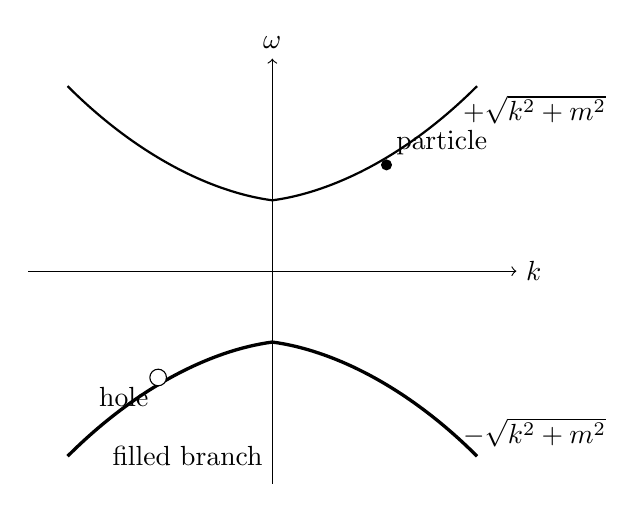
\begin{tikzpicture}[scale=1.0]
\draw[->] (-3.1,0) -- (3.1,0) node[right] {$k$};
\draw[->] (0,-2.7) -- (0,2.7) node[above] {$\omega$};
\draw[thick] (-2.6,2.35)
  .. controls (-1.7,1.45) and (-0.75,1.0) .. (0,0.9)
  .. controls (0.75,1.0) and (1.7,1.45) .. (2.6,2.35);
\draw[very thick] (-2.6,-2.35)
  .. controls (-1.7,-1.45) and (-0.75,-1.0) .. (0,-0.9)
  .. controls (0.75,-1.0) and (1.7,-1.45) .. (2.6,-2.35);
\fill (1.45,1.35) circle (2pt);
\node[above right] at (1.45,1.35) {particle};
\fill[white] (-1.45,-1.35) circle (3pt);
\draw (-1.45,-1.35) circle (3pt);
\node[below left] at (-1.45,-1.35) {hole};
\node[right] at (2.3,2.05) {$+\sqrt{k^2+m^2}$};
\node[right] at (2.3,-2.05) {$-\sqrt{k^2+m^2}$};
\node[left] at (0,-2.35) {filled branch};
\end{tikzpicture}
\caption{À tout moment, le spectre massif comporte des états d’énergie positive et négative. La branche négative est remplie ; un état manquant dans cette branche est un trou d’énergie positive.}
\end{figure}
À chaque moment correspond un état d’énergie positive et un état d’énergie négative. Le remplissage de tous les états de la branche négative laisse des particules d’énergie positive au-dessus de la mer et des trous d’énergie positive en son sein. Particules et trous ont tous deux une masse positive.

Le point essentiel mérite d’être répété. Un fermion acquiert une masse lorsque ses deux composantes, auparavant indépendantes, sont couplées. Au repos, aucune des deux composantes initiales n’est à elle seule un état propre de l’énergie. Les états d’énergie bien définie sont leur somme et leur différence.

Pour comprendre ce que signifie la somme, notons \(C_R^\dagger\) et \(C_L^\dagger\) les opérateurs de création pertinents pour une particule. Agissant sur le vide,
\begin{equation}
(C_R^\dagger+C_L^\dagger)\lvert0\rangle
\end{equation}
elle crée une particule dans une superposition cohérente des deux composantes. Elle n’en crée pas deux. Un produit,
\begin{equation}
C_R^\dagger C_L^\dagger\lvert0\rangle,
\end{equation}
contient deux opérateurs de création et crée un état à deux particules lorsque les deux modes sont disponibles. Après normalisation, l’état au repos a une probabilité égale pour chacune des deux composantes, mais l’onde couplée dans son ensemble a un moment nul.

Les étiquettes \(R\) et \(L\) ne désignaient un mouvement au sens littéral que lorsque \(m=0\). Dès que le terme de masse est présent, une solution massive en mouvement comporte généralement les deux composantes, et la solution au repos les comporte avec la même amplitude. Il est donc préférable de considérer ici \(R\) et \(L\) comme des désignations des composantes supérieure et inférieure du spineur.

\begin{figure}[htbp]
\centering
\includegraphics[width=0.78\textwidth]{lecture_06_figure_04.png}
\caption{Pour une masse non nulle, les deux composantes du spineur sont couplées ; leur interprétation en termes de mouvement vers la droite ou vers la gauche ne s’applique directement que dans la limite sans masse.}
\lectureframe{00:50:48}
\end{figure}

En physique des particules, tous les fermions massifs sont construits à partir de champs de composantes gauche et droite : une masse de Dirac couple des composantes indépendantes dans la limite sans masse.

\begin{classroomqa}
\lecturetimestamp{00:52:01}
\audiencequestion{Faut-il inclure un facteur \(1/\sqrt{2}\) dans \(\psi_R\pm\psi_L\) ?}
\lecturerresponse{On peut l’inclure pour normaliser l’état. Il multiplie les deux membres de l’équation et ne modifie donc pas l’équation du mouvement.}
\end{classroomqa}

\begin{classroomqa}
\lecturetimestamp{00:52:12}
\audiencequestion{Les amplitudes relatives des composantes droite et gauche ont-elles de l’importance ?}
\lecturerresponse{Pour les états propres au repos considérés ici, elles sont égales. La normalisation globale est arbitraire, mais les amplitudes relatives sont fixées par le vecteur propre de \(\beta\).}
\end{classroomqa}

\begin{classroomqa}
\lecturetimestamp{00:52:52}
\audiencequestion{Les deux composantes peuvent-elles avoir une phase relative ?}
\lecturerresponse{Oui. Les coefficients réels dans \(\psi_R\pm\psi_L\) découlent du choix d’une matrice \(\beta\) réelle. D’autres matrices qui vérifient les mêmes relations de carré égal à l’identité et d’anticommutation avec \(\alpha\) constituent des choix équivalents ; des phases relatives entre les composantes peuvent alors apparaître. Une fois une représentation choisie, il faut l’utiliser de manière cohérente.}
\end{classroomqa}

\begin{classroomqa}
\lecturetimestamp{00:53:43}
\audiencequestion{Les expressions ``mode se déplaçant vers la gauche'' et ``mode se déplaçant vers la droite'' deviennent-elles trompeuses lorsqu’on ajoute une masse ?}
\lecturerresponse{Dans une certaine mesure. Elles décrivent bien des ondes se déplaçant vers la gauche ou vers la droite dans la théorie sans masse. Avec une masse non nulle, même une particule qui se déplace dans une seule direction comporte généralement les deux composantes ; ``composante supérieure'' et ``composante inférieure'' sont donc des désignations plus sûres.}
\end{classroomqa}

\begin{classroomqa}
\lecturetimestamp{00:55:01}
\audiencequestion{Un fermion au repos a-t-il déjà besoin d’un moment cinétique de spin ?}
\lecturerresponse{Pas dans ce modèle à une dimension. Le moment cinétique n’est pas défini dans une dimension spatiale ; le spin n’intervient donc pas encore dans la construction.}
\end{classroomqa}

\begin{classroomqa}
\lecturetimestamp{00:55:24}
\audiencequestion{La fonction d’onde contient-elle des opérateurs fermioniques de création et d’annihilation ?}
\lecturerresponse{Oui.}
\end{classroomqa}

\begin{classroomqa}
\lecturetimestamp{00:55:30}
\audiencequestion{En quoi le caractère fermionique intervient-il, en dehors du choix des opérateurs de création et d’annihilation ?}
\lecturerresponse{Il intervient dans les règles fermioniques de création--et d’annihilation. Une équation présentant ce spectre d’énergie négative doit être quantifiée selon ces règles ; les règles d’occupation bosoniques laisseraient le vide instable. Les bosons relativistes doivent être décrits par une autre équation d’onde.}
\end{classroomqa}

\begin{classroomqa}
\lecturetimestamp{00:56:20}
\audiencequestion{Peut-on transformer par une transformation de Lorentz une solution à moment non nul en la solution au repos ?}
\lecturerresponse{Oui. Une transformation de Lorentz peut amener une solution massive dans son référentiel au repos, mais pour effectuer cette transformation, il faut connaître l’action des transformations de Lorentz sur le spineur \(\Psi\).}
\end{classroomqa}

\section{La masse issue d’un champ scalaire dans le vide}

\begin{classroomqa}
\lecturetimestamp{00:58:11}
\audiencequestion{Comment l’interaction avec le champ de Higgs produit-elle le terme de masse de Dirac ?}
\lecturerresponse{On remplace le coefficient de masse constant par un couplage à un champ scalaire. Si ce champ s’annule dans le vide, le fermion reste sans masse ; s’il prend une valeur constante non nulle dans le vide, le couplage agit exactement comme une masse.}
\end{classroomqa}

Soit \(\phi(x,t)\) un champ scalaire doté de sa propre équation du mouvement. Dans l’équation de Dirac, remplaçons la constante \(m\) du terme de masse par \(g\phi(x,t)\) :\footnote{Le terme d’interaction affiché s’obtient en effectuant cette substitution dans le terme de masse établi précédemment \(m\beta\Psi\).}\begin{equation}
i\frac{\partial\Psi}{\partial t}
=
-i\alpha\frac{\partial\Psi}{\partial x}
+g\phi(x,t)\,\beta\Psi.
\end{equation}
Les deux équations de champ sont alors couplées. Le fermion agit sur le champ scalaire, qui agit en retour sur le fermion ; considéré dans son ensemble, le système est non linéaire, bien que l’équation de Dirac soit linéaire en \(\Psi\) pour un champ \(\phi\) donné.

Supposons d’abord que le vide ait pour valeur
\begin{equation}
\phi(x,t)=0.
\end{equation}
Le terme de mélange s’annule alors, les composantes supérieure et inférieure se découplent et le fermion est sans masse. Supposons plutôt que l’état de plus basse énergie ait un champ scalaire constant non nul,
\begin{equation}
\phi(x,t)=\phi_0\neq0.
\end{equation}
Dans ce vide, l’équation de Dirac devient
\begin{equation}
i\frac{\partial\Psi}{\partial t}
=
-i\alpha\frac{\partial\Psi}{\partial x}
+g\phi_0\,\beta\Psi,
\end{equation}
donc
\begin{equation}
m_{\mathrm{eff}}=g\phi_0.
\end{equation}
Un couplage entre un champ bosonique et un champ fermionique, associé à une valeur non nulle du champ bosonique dans le vide, produit donc le même mélange entre les composantes gauche et droite que celui qui apparaissait auparavant sous la forme d’une masse inscrite directement dans l’équation.

\begin{classroomqa}
\lecturetimestamp{01:01:27}
\audiencequestion{Le LHC pourrait-il fournir des indices en faveur d’un champ de Higgs non nul dans le vide ?}
\lecturerresponse{Absolument. C’est l’une des grandes questions.}
\end{classroomqa}

\begin{classroomqa}
\lecturetimestamp{01:01:32}
\audiencequestion{Pouvez-vous expliquer davantage le fonctionnement du mécanisme de Higgs ?}
\lecturerresponse{Un champ scalaire possède une énergie associée à ses variations spatiales et temporelles ; il peut aussi avoir une énergie potentielle locale \(V(\phi)\). Si les minima de ce potentiel se trouvent à des valeurs non nulles de \(\phi\), le vide contient un champ non nul. Les oscillations quantifiées autour du minimum choisi sont des particules de Higgs.}
\end{classroomqa}

Un champ peut porter de l’énergie de deux manières distinctes. Une partie de l’énergie dépend de la façon dont le champ varie dans l’espace et le temps. Le champ de Maxwell fournit un exemple familier :
\begin{equation}
\mathcal{E}_{\mathrm{Maxwell}}\propto \mathbf E^2+\mathbf B^2,
\end{equation}
et \(\mathbf E\) comme \(\mathbf B\) sont construits à partir des dérivées du potentiel électromagnétique. Cette énergie est donc liée aux variations spatiales et temporelles du champ sous-jacent.

Un champ scalaire peut aussi avoir une densité locale d’énergie potentielle,
\begin{equation}
V(\phi),
\end{equation}
qui dépend de la valeur de \(\phi\) elle-même, plutôt que de ses dérivées. Schématiquement,
\begin{equation}
\mathcal{E}_\phi
=
\mathcal E_{\text{space and time gradients}}+V(\phi).
\end{equation}
En l’absence d’un principe plus profond qui la détermine, \(V(\phi)\) pourrait être n’importe quelle fonction raisonnable compatible avec les symétries du modèle.

Pour l’illustration simplifiée utilisée ici, avec un champ scalaire réel, supposons que la théorie soit invariante sous la transformation
\begin{equation}
\phi\longrightarrow-\phi.
\end{equation}
Le potentiel doit alors être une fonction paire :
\begin{equation}
V(\phi)=V(-\phi).
\end{equation}
Cette symétrie ne précise pas, à elle seule, où se trouve le minimum. Il peut y avoir un minimum unique en \(\phi=0\), ou bien deux minima symétriques à des valeurs non nulles, l’un positif et l’autre négatif.

\begin{figure}[htbp]
\centering
\includegraphics[width=0.72\textwidth]{lecture_06_figure_05.png}
\caption{Un minimum en \(\phi=0\) correspond à un champ nul dans le vide, tandis que des minima symétriques non nuls permettent une valeur de vide \(\phi_0\neq0\) et, par conséquent, une masse fermionique \(g\phi_0\).}
\lectureframe{01:04:47}
\end{figure}

On peut représenter les deux possibilités sans choisir une forme polynomiale particulière pour le potentiel.\footnote{Les courbes ci-dessous ne montrent que les minima qualitatifs centrés et liés par symétrie utilisés dans l’argument.}
\begin{figure}[htbp]
\centering
\resizebox{\linewidth}{!}{%
\begin{tikzpicture}[x=1.35cm,y=1.05cm]
\begin{scope}[shift={(-3.1,0)}]
\draw[->] (-1.7,0) -- (1.7,0) node[right] {$\phi$};
\draw[->] (0,-0.15) -- (0,2.45) node[above] {$V(\phi)$};
\draw[thick] (-1.5,2.05) .. controls (-0.9,0.65) and (-0.45,0.25) .. (0,0.25)
             .. controls (0.45,0.25) and (0.9,0.65) .. (1.5,2.05);
\fill (0,0.25) circle (1.2pt);
\node[below] at (0,0) {$0$};
\end{scope}
\begin{scope}[shift={(3.1,0)}]
\draw[->] (-1.7,0) -- (1.7,0) node[right] {$\phi$};
\draw[->] (0,-0.15) -- (0,2.45) node[above] {$V(\phi)$};
\draw[thick] (-1.55,2.05)
  .. controls (-1.25,0.75) and (-1.0,0.25) .. (-0.75,0.25)
  .. controls (-0.35,0.25) and (-0.25,1.3) .. (0,1.3)
  .. controls (0.25,1.3) and (0.35,0.25) .. (0.75,0.25)
  .. controls (1.0,0.25) and (1.25,0.75) .. (1.55,2.05);
\fill (-0.75,0.25) circle (1.2pt);
\fill (0.75,0.25) circle (1.2pt);
\node[below] at (0,0) {$0$};
\node[below] at (-0.75,0) {$-\phi_0$};
\node[below] at (0.75,0) {$\phi_0$};
\end{scope}
\end{tikzpicture}%
}
\caption{Un potentiel pair peut avoir un minimum centré ou deux minima non nuls liés par symétrie.}
\end{figure}

Si le minimum se trouve à l’origine, le vide a pour valeur \(\phi_0=0\), et ce couplage ne donne aucune masse à l’électron. Si les minima sont en \(\phi=\pm\phi_0\), le vide se stabilise dans l’un ou l’autre. Ces deux choix sont liés par la symétrie et produisent chacun un coefficient non nul \(g\phi_0\) dans l’équation de Dirac. La raison pour laquelle le potentiel a cette forme qualitative est une question plus profonde, à laquelle le mécanisme lui-même ne répond pas.

Le champ n’a pas à rester exactement à son minimum. Il peut osciller autour de la valeur choisie, comme une particule peut osciller près du fond d’un puits de potentiel. La quantification de ces oscillations donne des quanta de Higgs. Leur fréquence caractéristique est liée à la masse de la particule de Higgs : une masse élevée signifie qu’il faut une grande quantité d’énergie pour exciter ne serait-ce qu’un quantum. Dans le vide, le champ reste simplement près de son minimum et fournit la masse du fermion. Lorsque le champ vibre, cette vibration est une particule de Higgs.

Le couplage entraîne une action réciproque. Les fermions réagissent à la valeur de \(\phi\), mais des collisions de fermions suffisamment énergétiques peuvent aussi exciter le champ scalaire. Une collision doit fournir l’énergie nécessaire à l’excitation ; une fois le champ en vibration, ses quanta sont des particules de Higgs. Ce même champ se couple non seulement aux électrons, mais aussi aux champs de quarks et à d’autres champs auxquels il donne une masse.

\begin{classroomqa}
\lecturetimestamp{01:08:14}
\audiencequestion{La masse de l’électron change-t-elle si le champ de Higgs vibre ou s’écarte de sa valeur de vide ?}
\lecturerresponse{Oui. Comme la masse effective est proportionnelle à la valeur locale du champ, un déplacement du champ vers zéro réduit la masse. Maintenir une région macroscopique loin de la valeur de vide exigerait une énergie énorme ; une région assez grande pour une telle expérience pourrait s’effondrer en trou noir.}
\end{classroomqa}

L’expérience de pensée est simple. Si l’on pouvait maintenir une région près de \(\phi=0\), alors, dans cette région,
\begin{equation}
m_{\mathrm{eff}}=g\phi
\end{equation}
diminuerait ou s’annulerait. Un mode de Higgs excité oscille autour de la valeur de vide, tandis que produire et maintenir un écart appréciable dans toute une région macroscopique exige une énergie énorme. Le coût en énergie potentielle augmente avec le volume. Bien avant qu’une telle région puisse servir de laboratoire pratique, son énergie pourrait être assez élevée pour provoquer un effondrement gravitationnel. En principe, la masse change réellement, mais obtenir une variation importante et observable est extraordinairement difficile.

\begin{classroomqa}
\lecturetimestamp{01:09:27}
\audiencequestion{Pourquoi faut-il un champ de Higgs ?}
\lecturerresponse{Parce que l’électron a une masse.}
\end{classroomqa}

\begin{classroomqa}
\lecturetimestamp{01:09:41}
\audiencequestion{Chaque type de particule a-t-il son propre champ de Higgs ?}
\lecturerresponse{Non. Dans le Modèle standard, un seul champ de Higgs fournit leur masse aux électrons, aux quarks et aux autres particules concernées par ce mécanisme. Les versions supersymétriques requièrent deux champs de Higgs, plutôt qu’un champ distinct pour chaque espèce de particule.}
\end{classroomqa}

L’image d’un champ unique est schématique : le champ de Higgs complet a une structure plus riche qu’un seul nombre réel \(\phi\). Le point essentiel demeure néanmoins valable. Un champ de vide commun peut se coupler avec des intensités différentes aux divers fermions ; des masses différentes n’exigent donc pas un champ de Higgs distinct pour chaque espèce. La particule de Higgs est une oscillation de ce même champ autour de sa valeur de vide.

Pourquoi ne pas simplement introduire à la main la masse de l’électron dans l’équation et se passer du champ de Higgs ? La réponse concerne les interactions faibles et l’unification ; nous y reviendrons plus tard.

\begin{classroomqa}
\lecturetimestamp{01:11:16}
\audiencequestion{Dans une théorie supersymétrique, y a-t-il deux secteurs de Higgs ?}
\lecturerresponse{Oui. Dans la distinction simplifiée présentée ici, l’un fournit leur masse aux quarks de type haut et l’autre aux quarks de type bas et aux électrons. Ce dédoublement est une exigence technique de la supersymétrie, et non l’introduction d’un champ de Higgs distinct pour chaque particule.}
\end{classroomqa}

\begin{classroomqa}
\lecturetimestamp{01:12:01}
\audiencequestion{Si la particule de Higgs a une masse, d’où vient-elle ?}
\lecturerresponse{Cette question n’est pas résolue ici. L’énigme plus précise est de savoir pourquoi la masse du Higgs est si faible.}
\end{classroomqa}

La symétrie est indissociable de la question de la masse. Dans le modèle de Dirac simple, une symétrie qui empêche les secteurs gauche et droit de se mélanger imposerait l’annulation du coefficient du terme de mélange. Si le vide respectait cette symétrie, le fermion serait sans masse. Une valeur non nulle du champ de Higgs dans le vide brise la symétrie correspondante du vide et permet le couplage entre les secteurs gauche et droit :
\begin{equation}
m_{\mathrm{eff}}=g\phi_0\neq0.
\end{equation}
La transformation de symétrie précise n’est pas développée ici ; c’est sa conséquence pour le terme de masse qui importe. Les équations peuvent posséder cette symétrie même si l’état particulier de plus basse énergie ne la possède pas. C’est cette asymétrie du vide qui fournit la masse.

Dans le cadre électrofaible esquissé ici, les électrons et les quarks acquièrent ainsi une masse, tout comme les bosons \(W\) et \(Z\). Le photon reste sans masse. La particule de Higgs elle-même constitue une autre exception : elle peut avoir une masse même en l’absence du même déplacement du vide, et sa masse est liée aux oscillations de son propre champ plutôt qu’au mélange gauche-droite des fermions. Ainsi, dans cette description, la valeur du champ de Higgs dans le vide engendre les masses des autres particules, tandis que la masse de l’excitation de Higgs soulève une question distincte.

\begin{classroomqa}
\lecturetimestamp{01:15:26}
\audiencequestion{Le graviton a-t-il une masse ?}
\lecturerresponse{Non. Le graviton est sans masse, comme le photon. On pensait autrefois que les neutrinos étaient eux aussi sans masse, mais ils ont une masse très faible ; dans le langage employé ici, cela signifie que leurs composantes gauche et droite ne sont que très faiblement couplées.}
\end{classroomqa}

Les photons et, selon la théorie, les gravitons sont sans masse et se déplacent à la vitesse de la lumière. Les neutrinos n’appartiennent pas tout à fait à cette catégorie. Leur masse infime signifie, dans ce langage de Dirac, que le couplage entre leurs composantes gauche et droite est infime. La raison de cette faiblesse est une autre question.

\section{L’équation de Dirac en trois dimensions spatiales}

En trois dimensions spatiales, le nombre d’onde devient un vecteur d’onde,
\begin{equation}
\mathbf{k}=(k_1,k_2,k_3),
\end{equation}
avec des composantes selon les directions \(x\), \(y\) et \(z\). En une dimension, la relation prend la forme
\begin{equation}
\omega=\alpha k+\beta m,
\end{equation}
et sa généralisation linéaire la plus simple est
\begin{equation}
\omega
=
\alpha_1 k_1+\alpha_2 k_2+\alpha_3 k_3+\beta m.
\end{equation}
Ici, \(\alpha_i\) et \(\beta\) sont des matrices. Elles doivent être choisies de façon que
\begin{equation}
\omega^2=k_1^2+k_2^2+k_3^2+m^2.
\end{equation}
Cette relation de dispersion invariante est une condition essentielle, même si elle ne suffit pas, à elle seule, à rendre compte de toute la relativité.

Le carré de l’expression linéaire donne
\begin{align}
\omega^2
={}&
\alpha_1^2k_1^2+\alpha_2^2k_2^2+\alpha_3^2k_3^2+\beta^2m^2
\nonumber\\
&+(\alpha_1\alpha_2+\alpha_2\alpha_1)k_1k_2
+(\alpha_1\alpha_3+\alpha_3\alpha_1)k_1k_3
\nonumber\\
&+(\alpha_2\alpha_3+\alpha_3\alpha_2)k_2k_3
+\sum_{i=1}^{3}(\alpha_i\beta+\beta\alpha_i)k_i m.
\end{align}
Les coefficients des carrés des moments et de la masse doivent satisfaire
\begin{equation}
\alpha_1^2=\alpha_2^2=\alpha_3^2=I,
\qquad
\beta^2=I.
\end{equation}
Les termes indésirables \(k_i k_j\) s’annulent si les matrices \(\alpha\) distinctes anticommutent :
\begin{equation}
\alpha_i\alpha_j+\alpha_j\alpha_i=0,
\qquad i\neq j.
\end{equation}
Les termes croisés \(k_i m\) s’annulent si
\begin{equation}
\alpha_i\beta+\beta\alpha_i=0
\qquad
\text{for each }i.
\end{equation}
Les quatre matrices ont donc toutes pour carré l’identité, et deux matrices distinctes quelconques anticommutent.

Il existe bien trois matrices \(2\times2\) qui possèdent les propriétés d’anticommutation mutuelle requises : ce sont les trois matrices de Pauli. Il n’existe pas de quatrième matrice \(2\times2\) dont le carré soit l’identité et qui anticommuterait avec les trois autres. Aucune réalisation \(3\times3\) ne convient non plus. La plus petite réalisation possible fait intervenir des matrices \(4\times4\) : les matrices de Dirac.

Le passage de deux à quatre composantes soulève une question physique. En une dimension spatiale, les deux composantes représentaient au départ des champs se propageant vers la droite et vers la gauche. Que signifient quatre composantes ? Le nouvel élément sera le spin, mais celui-ci suppose un moment cinétique et exige donc une véritable discussion en trois dimensions.

Les matrices ne sont pas uniques. Des choix différents sont équivalents, à peu près comme le sont différents choix d’axes de coordonnées mutuellement orthogonaux : les éléments changent, mais une transformation relie les descriptions, sans modifier la physique. Une représentation commode est\footnote{Les matrices écrites élément par élément ci-dessous sont le développement de la forme par blocs et des matrices de Pauli présentées juste après ; ces relations entre blocs sont énoncées explicitement dans le cours à 013023--013129.}
\begin{equation}
\beta=
\begin{pmatrix}
1&0&0&0\\
0&1&0&0\\
0&0&-1&0\\
0&0&0&-1
\end{pmatrix},
\end{equation}
ainsi que
\begin{align}
\alpha_1&=
\begin{pmatrix}
0&0&0&1\\
0&0&1&0\\
0&1&0&0\\
1&0&0&0
\end{pmatrix},
&
\alpha_2&=
\begin{pmatrix}
0&0&0&-i\\
0&0&i&0\\
0&-i&0&0\\
i&0&0&0
\end{pmatrix},
\\[1ex]
\alpha_3&=
\begin{pmatrix}
0&0&1&0\\
0&0&0&-1\\
1&0&0&0\\
0&-1&0&0
\end{pmatrix}.
\end{align}
Leur structure apparaît plus clairement si l’on décompose chaque matrice en blocs \(2\times2\) :
\begin{equation}
\beta=
\begin{pmatrix}
I_2&0\\
0&-I_2
\end{pmatrix},
\qquad
\alpha_i=
\begin{pmatrix}
0&\sigma_i\\
\sigma_i&0
\end{pmatrix}.
\end{equation}
Les trois matrices de Pauli sont
\begin{equation}
\sigma_1=
\begin{pmatrix}
0&1\\
1&0
\end{pmatrix},
\quad
\sigma_2=
\begin{pmatrix}
0&-i\\
i&0
\end{pmatrix},
\quad
\sigma_3=
\begin{pmatrix}
1&0\\
0&-1
\end{pmatrix}.
\end{equation}
Ces matrices par blocs satisfont aux relations d’anticommutation requises pour les matrices de Dirac.

La fonction d’onde doit maintenant avoir quatre composantes :
\begin{equation}
\Psi=
\begin{pmatrix}
\psi_1\\
\psi_2\\
\psi_3\\
\psi_4
\end{pmatrix}.
\end{equation}
L’équation du mouvement est
\begin{equation}
i\frac{\partial\Psi}{\partial t}
=
-i\sum_{j=1}^{3}\alpha_j
\frac{\partial\Psi}{\partial x_j}
+\beta m\Psi.
\end{equation}
Cette expression compacte représente quatre équations différentielles linéaires couplées. Les éléments hors diagonale des matrices \(\alpha_j\) mélangent les quatre composantes de manière plus complexe que dans le cas unidimensionnel, mais la structure fondamentale est la même : les matrices couplent les composantes, tandis que l’équation reste du premier ordre en espace et en temps. Le doublement supplémentaire du nombre de composantes met sur la piste du spin.

\begin{classroomqa}
\lecturetimestamp{01:33:53}
\audiencequestion{Les quatre composantes de \(\Psi\) forment-elles un quadrivecteur directement associé aux quatre dimensions de l’espace-temps ?}
\lecturerresponse{Non. Elles forment un spineur, pas un quadrivecteur. La correspondance entre les deux dimensions de l’espace-temps et les deux composantes du spineur dans l’exemple unidimensionnel était fortuite. Dans les constructions en dimensions supérieures, les dimensions des matrices de spineurs sont des puissances de deux et ne coïncident généralement pas avec le nombre de dimensions de l’espace-temps.}
\end{classroomqa}

Le référentiel au repos fournit de nouveau l’interprétation la plus simple. À quantité de mouvement nulle, le terme dérivé s’annule :
\begin{equation}
i\frac{\partial\Psi}{\partial t}=m\beta\Psi.
\end{equation}
Dans la représentation choisie, \(\beta\) a deux valeurs propres \(+1\) et deux valeurs propres \(-1\). Il y a donc deux états au repos d’énergie \(+m\) et deux d’énergie \(-m\). Comme précédemment, les états d’énergie négative sont remplis. La multiplicité double de chaque signe de l’énergie constitue la structure supplémentaire dont l’interprétation physique est le spin.

\begin{classroomqa}
\lecturetimestamp{01:35:51}
\audiencequestion{Les blocs hors diagonale de \(\alpha_i\) doivent-ils porter le même indice, de sorte qu’il s’agisse de \(\sigma_i\) ?}
\lecturerresponse{Oui. Chaque matrice \(\alpha_i\) contient la matrice de Pauli correspondante \(\sigma_i\) dans chacun de ses deux blocs hors diagonale.}
\end{classroomqa}

\begin{classroomqa}
\lecturetimestamp{01:36:03}
\audiencequestion{Manque-t-il un facteur deux dans la relation compacte d’anticommutation des \(\alpha_i\) ?}
\lecturerresponse{Oui. Lorsque \(i=j\), le membre de gauche vaut \(\alpha_i^2+\alpha_i^2=2I\). La relation correcte est \(\alpha_i\alpha_j+\alpha_j\alpha_i=2\delta_{ij}I\).}
\end{classroomqa}

On peut donc réunir les conditions portant séparément sur le carré et sur les indices distincts sous la forme
\begin{equation}
\alpha_i\alpha_j+\alpha_j\alpha_i=2\delta_{ij}I.
\end{equation}

\begin{classroomqa}
\lecturetimestamp{01:36:42}
\audiencequestion{Le passage à quatre matrices a-t-il constitué un grand saut conceptuel dans la construction de Dirac ?}
\lecturerresponse{Oui. Dirac a postulé l’équation, puis en a tiré les conséquences. L’une d’elles était l’existence des antiparticules ; une autre, celle du spin. Le spin était déjà connu empiriquement, mais l’équation en rendait compte.}
\end{classroomqa}

\begin{classroomqa}
\lecturetimestamp{01:37:29}
\audiencequestion{Qu’est-ce qui est venu en premier : les observations empiriques ou le théorème limitant les particules aux bosons et aux fermions ?}
\lecturerresponse{Les observations empiriques sont venues en premier, et le théorème plus tard. L’alternative boson--fermion s’applique en trois dimensions spatiales. En deux dimensions spatiales et une dimension temporelle, des statistiques intermédiaires peuvent apparaître ; en dimensions \(3+1\) et dans les dimensions spatiales supérieures, les possibilités sont les bosons et les fermions.}
\end{classroomqa}

\begin{classroomqa}
\lecturetimestamp{01:39:01}
\audiencequestion{Existe-t-il une convention pour indexer les quatre composantes de \(\Psi\) ?}
\lecturerresponse{Aucun choix particulier n’est imposé ici. On peut utiliser les indices \(p\) et \(q\), allant de un à quatre ; chaque matrice a alors un indice de ligne et un indice de colonne.}
\end{classroomqa}

La notation matricielle omet ces indices de composantes. Si on les fait apparaître, on obtient
\begin{equation}
p,q=1,2,3,4,
\end{equation}
et l’équation s’écrit
\begin{equation}
i\,\partial_t\Psi_p
=
-i\sum_{j=1}^{3}\sum_{q=1}^{4}
(\alpha_j)_{pq}\,\partial_j\Psi_q
+m\sum_{q=1}^{4}\beta_{pq}\Psi_q.
\end{equation}

\begin{classroomqa}
\lecturetimestamp{01:40:15}
\audiencequestion{Les indices explicites des composantes sont-ils superflus lorsqu’on utilise la multiplication matricielle ?}
\lecturerresponse{Oui. La notation matricielle omet automatiquement ces indices. On pourra introduire plus tard une forme plus symétrique, qui rendra la structure relativiste plus explicite.}
\end{classroomqa}

L’équation présentée est l’équation de Dirac dans sa forme la plus simple en \(3+1\) dimensions. Les prochaines étapes consistent à comprendre le spin et à construire les équations d’onde des bosons relativistes, puisque l’équation de Dirac n’est pas la leur et qu’environ la moitié des particules de la nature sont des bosons. Une fois ces éléments en place, on pourra aborder les quarks, les leptons, les bosons faibles, les particules de Higgs et les photons, et mettre un peu d’ordre dans le spectre des particules. Une symétrie plus étendue sera nécessaire tout au long de cette discussion.
